\documentclass[12,a4paper]{article}
\usepackage{fontspec}
\usepackage{geometry}
\usepackage{fontspec}
\usepackage{xeCJK}
\usepackage{amsmath}
\usepackage{fancyhdr}
\usepackage{physics}
\usepackage{tikz}
\usepackage{graphicx}
\usepackage{placeins}
\usetikzlibrary{positioning}
\setCJKmainfont{標楷體}
\XeTeXlinebreaklocale "zh"
\XeTeXlinebreakskip = 0pt plus 1pt
\geometry{a4paper,scale=0.8}
\pagestyle{fancy}
\fancyhf{}
\rhead{Artificial-Intelligence}
\lhead{張紳濡}
\cfoot{\thepage}
\title{{\Huge Artificial-Intelligence} \\ homework2 }
\author{0816023 張紳濡}
\date{}
\begin{document}
\maketitle
\thispagestyle{fancy}
\section{Introduction}
使用Bi-gram與DistilBert偵測正面與負面評論
\section{Data}
\begin{itemize}
\item train: 20000 positive and 20000 negative review.
\item test: 5000 positive and 5000 negative review.
\end{itemize}
\section{What I do}
\subsection{Preprocessing}
\begin{itemize}
    \item function 1: remove chinese words:\\
        e.g.:\\
        'War movie' is a Hollywood genre that has been done and redone so many times that clich矇d dialogue \\
        -> ' War movie ' Hollywood genre done redone many times clichd dialogue
    \item function 2: remove Punctuation:\\
        e.g.:\\
        .<br /><br />My intention to see it was certainly JJL being one of my favourite actresses. \\
        ->My intention see certainly JJL one favourite actresses
    \item function 3: remove number:\\
        e.g.:\\
        I saw this movie when I was about 12 when it came out.\\
        ->saw movie  came
\end{itemize}
All of example have removed stop words
\subsection{Different numbers of feature-num}
這邊的feature-num我使用500與250,結果如下表:
\begin{figure}[!ht]
\centering
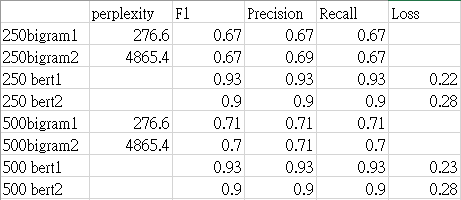
\includegraphics[width=0.8\textwidth]{pic/sheet1.png}
\end{figure}
\FloatBarrier
\begin{itemize}
    \item perplexity:在perplexity的部分,可以明顯發現在經過preprocessing後perplexity明顯上升,我想是因為去除了stop word與標點符號所以相似的bigram變少了(perplexity越小越好)這邊為了處理0的問題我把等於0的改成0.00001(smoothing)
    \item F1 score: 這邊在F1 score的部分,在bi gram比較能看得出差異 對於feautre-num為500的model F1 score略高一些代表對於bi gram 取比較多的feature會比較好,而bert方面我覺得可能250就足夠他判斷了。
    \item precision,recall: 可以發現precesion與recall還蠻平均的,代表model不會太過謹慎也不會太過寬鬆。
\end{itemize}
\subsection{Bi-gram VS DistilBert}
\begin{itemize}
    \item bi-gram cannot outperform DistilBert: 我認為是因為bert會考慮整個語句而bi-gram只考慮部分語句,而且bert有比較多層
    \item Can bi-gram consider long-term dependencies:我覺得可能可以把perplexity加入model的訓練內可能可以,因為perplexity有整句的資訊。
    \item Would the preprocessing methods improve the performance of the bi-gram model: 我覺得這次訓練下來的結果沒有增進結果,從上面的表格可以發現並沒有增進多少,我考慮過可能是我preprocessing沒做好因此跑過只移除stop word的版本如下表:
    \begin{figure}[!ht]
    \centering
    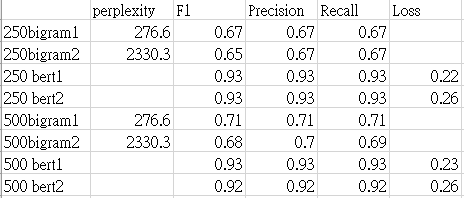
\includegraphics[width=0.8\textwidth]{pic/sheet2.png}
    \end{figure}
    \FloatBarrier
    可以發現也沒有增加多少。
    \item UNK: 我認為perplexity會減少,因為原本不同bigram但機率很低的bigram會整合在一起因而減少perplexity。
\end{itemize}
\section{Problem I meet}
\subsection{run too long}
在part 1 的部分若要做到example的結果需要跑很久,因為要生成每個word對映下一個word的機率表,而我在做其他部分的時候也沒有用到這個部分,因此我在跑的時候把這邊註解掉了(model.py line 60-65)
\subsection{preprocessing}
我認為preprocessing應該要讓結果變好,但實際上的結果並沒有,因此我認為可能有更好的preprocessing function可以實作使結果變好。
\section{Code}
All code can be find in\\
https://github.com/Sakuya0229/Artificial-Intelligence-HW2








\end{document}
